\section{User evaluation}\label{sec:userevaluation}

As a team we were advised by our project manager to perform a preliminary, in-house user test before the Project Discovery game would be showcased at EVE Vegas, a conference for EVE Online players and fans. The purpose of this test was to shed light on any obvious errors with the game, especially the tutorial phase which was at an early stage at the time.

\subsection{Implemention}
The tests took place on the 9th of October. We got five volunteers from CCP, four males and one female between the ages of 25 to 40. The people were a mix of game designers, quality assurance people and a community developer. The reason we only got people from within CCP to partake in the tests was that the game was not ready to be revealed to the public so we could not get people outside of CCP to perform the test.

The test was performed on a computer that remotely connected to our personal work desktop. When a tester arrived, we greeted them, thanked them for coming, and explained the procedure. The procedure was that the tester would sit down and we would observe them while they played. The player would open Project Discovery, finish the tutorial and a handful of other tasks. While playing, the tester would verbally express their thoughts, for us to write down. Testers could play for as long as they wanted, given that they continued to think aloud.

After the tester had finished playing we asked them questions about their experience playing the game and then thanked them for their contribution to the project.

\subsection{Data}

In this section we outline the data received from each of the testers, this data is comprised of a list of questions we asked the testers after the test was performed, and their answers.

\begin{table}[H]
\centering
\caption{The first question}
\label{tab:question1}
\begin{tabular}{p{1.3cm}p{10cm}}
\toprule
 & \multicolumn{1}{c}{Did you find the tutorial helpful?} \\ \midrule
Tester 1 & \multicolumn{1}{c}{NA} \\
Tester 2 & Yes, but it was way too simple compared to the real game. \\
Tester 3 & No, I breezed through it and didn't pay attention to it. \\
Tester 4 & Yes, I liked it. \\
Tester 5 & Yes, but I felt that it didn't scale up in difficulty enough. \\ \bottomrule
\end{tabular}
\end{table}

\begin{table}[H]
\centering
\caption{The second question}
\label{tab:question2}
\begin{tabular}{p{1.3cm}p{10cm}}
\toprule
 & \multicolumn{1}{c}{Did you understand the aim of the game?} \\ \midrule
Tester 1 & Yes. \\
Tester 2 & Yes. \\
Tester 3 & No. \\
Tester 4 & Yes. \\
Tester 5 & Yes. \\ \bottomrule
\end{tabular}
\end{table}

\begin{table}[H]
\centering
\caption{The third question}
\label{tab:question3}
\begin{tabular}{p{1.3cm}p{10cm}}
\toprule
 & \multicolumn{1}{c}{Did you feel a sense of accomplishment when you were correct?} \\ \midrule
Tester 1 & Sure, it's pretty hard to get it right, but rewarding when you do. \\
Tester 2 & It's okay, I thought the result screen could show some more fanfare if you are correct. \\
Tester 3 & I did not feel accomplished. \\
Tester 4 & Yes! \\
Tester 5 & Yeah totally! It's always fun to be 100\% correct. \\ \bottomrule
\end{tabular}
\end{table}

\begin{table}[H]
\centering
\caption{The fourth question}
\label{tab:question4}
\begin{tabular}{p{1.3cm}p{10cm}}
\toprule
 & \multicolumn{1}{c}{Do you think the interface was easy to understand?} \\ \midrule
Tester 1 & Yes, but the color selection channels were not explained, so I didn't know what they were for. \\
Tester 2 & Yes. \\
Tester 3 & Yes. \\
Tester 4 & Sure, I think it could have been explained a little more though. \\
Tester 5 & Yes. \\ \bottomrule
\end{tabular}
\end{table}

\begin{table}[H]
\centering
\caption{The fifth question}
\label{tab:question5}
\begin{tabular}{p{1.3cm}p{10cm}}
\toprule
 & Did you feel a sense of excitement when waiting to see if your answer was correct? \\ \midrule
Tester 1 & Yes. \\
Tester 2 & Yes. \\
Tester 3 & Yes. \\
Tester 4 & Yes. \\
Tester 5 & Yes. \\ \bottomrule
\end{tabular}
\end{table}

\begin{table}[H]
\centering
\caption{The sixth question}
\label{tab:question5}
\begin{tabular}{p{1.3cm}p{10cm}}
\toprule
 & \multicolumn{1}{c}{Any thoughts or comments?} \\ \midrule
Tester 1 & Overall I thought it was really great, just a bit confusing at first. \\
Tester 2 & The tooltips were too long and technical, so I ignored them. I really would have liked to be able to zoom in on the main image. \\
Tester 3 & I would like a better tutorial, more information on what I should have been doing. \\
Tester 4 & I would like a zoom feature for the images. \\
Tester 5 & A zoom function would have been great, and simpler tutorial tooltips. \\ \bottomrule
\end{tabular}
\end{table}


\subsection{Results}

In this section we analyze the data we derived from the tests and how we used that data to come up with improvements for the game.

\subsubsection{Tooltips}
We gathered that proper use of tooltips was paramount to the players understanding of the game. Some players seemed to be confused about the objectives of the game. We saw that the tooltips needed to be clear and helpful to the players understanding the interface. So we decided that tooltips should be utilized when the players first see the interface, and also throughout the whole tutorial and training session, gradually teaching players about the game as they face the actual problems. The tooltips also needed to be shorter and focused on one specific message. Testers did not immediately grasp that they could change the colour filter on the main image, so we added a tooltip that describes this functionality.

\subsubsection{Tutorial}
Testers felt that the tutorial was too easy and did not teach them very much about the real game. To rectify this we implemented a more extensive tutorial, where each task teaches the player a specific aspect of the game. Such as explaining the interface, or how to classify certain patterns in images. 

Testers expressed the need for an explanation after each tutorial task, so we reached out to the researchers at The Human Protein Atlas to get explanations for each training task, and to explain why the correct solution was correct. We also enlisted their help in making the tutorial more focused and better at teaching players the skills needed to classify images.

\subsubsection{Interface}
Testers did not have much to say about the interface with the exception of everyone being in agreement that a magnificitation function was necessary on the main image. We responded to that by implementing a magnification function that allows players to zoom in to the full resolution of the main image within the image container and it gives players the option to fix the position of the zoomed in image so they can easily compare to the image to the categories available.

We observed that testers, who had completed the training phase, and were contributing to unknown tasks, did not get a result screen. That is normal behaviour since the solution is unknown, we can not reliably give a result. We saw that when users weren't getting instant feedback they were not as interested and seemed less motivated to find the right solution to the tasks. Our solution to this problem was that since we do know the community consensus for specific tasks at any given time, we can show exact percentages for choices by other players. We felt that since testers expressed excitement in seeing a result screen, we should implement this for unknown tasks, so that the game would not lose the factor of excitement once players reach the stage of solving images that have no known solution. To achieve this, instead of giving players a confirmed correct answer like we do with training tasks, we give players the current consensus of the task at the time the user submitted his solution. We also make sure to let players know that this consensus is not necessarily correct. That way the player can get a sense of what other players think the solution is and see if he's in agreement with them or not.

\begin{figure}[H]
	\centering
	\graphicspath{ {./graphics/} }
    \centerline{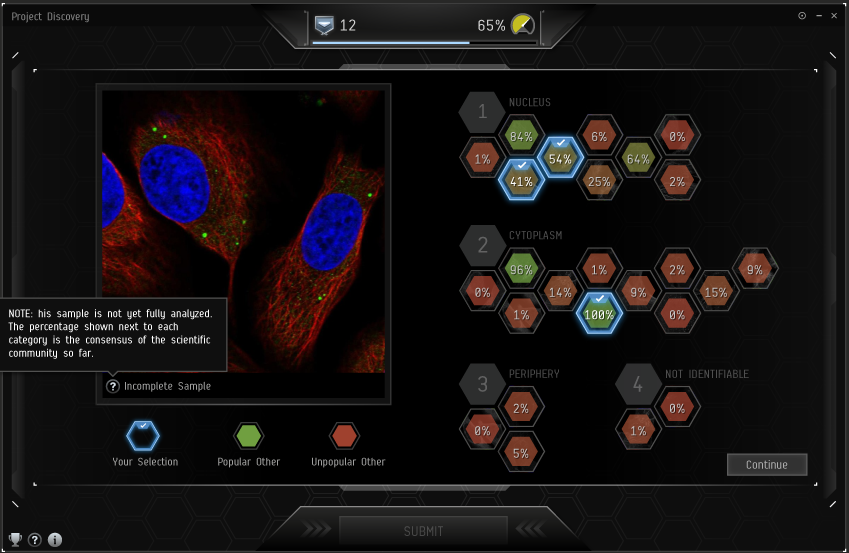
\includegraphics[scale=0.55]{unknow_result.png}}
    \caption{\label{fig:bdchart}A mockup of the consensus screen for unknown tasks}
\end{figure}